\documentclass{article}
\usepackage{amsmath, amssymb, amsthm} % For mathematical symbols and theorem environments
\usepackage[utf8]{inputenc}
\usepackage{graphicx} % Standard encoding

% LaTeX Note Title
\title{A Rotational Construction of Genus $g$ Surfaces from $(g-1)$ Octagons\\ Part 1: Fundamental Construction, Properties, and Further Remarks}

% Authors
\author{Mingli Yuan \and Gemini \and ChatGPT \and DeepSeek}

% Date
\date{\today}

% Theorem-like environments (optional, but good for structure)
\newtheorem{theorem}{Theorem}
\newtheorem{lemma}[theorem]{Lemma}
\newtheorem{proposition}[theorem]{Proposition}
\newtheorem{corollary}[theorem]{Corollary}
\theoremstyle{definition}
\newtheorem{definition}{Definition}
\newtheorem{example}{Example}
\theoremstyle{remark}
\newtheorem{remark}{Remark}

\begin{document}
\maketitle

\begin{abstract}
This note details a constructive method for orientable closed surfaces of genus $g \ge 2$. It leverages the concept of a genus $g$ surface $S_g$ as an $N=(g-1)$-sheeted $Z_N$-symmetric regular covering of a genus 2 surface $S_2$. We demonstrate that by gluing $N$ octagonal fundamental domains of $S_2$ according to specific rules derived from this covering structure, a surface of genus $g$ is indeed formed. This approach provides an alternative perspective to the standard construction of $S_g$ from a single $4g$-sided polygon and explicitly highlights the hierarchical relationship between $S_g$ and $S_2$. We present the general construction, a proof of its resulting genus using Euler characteristics, and illustrate it with a detailed example for $g=4$.
\end{abstract}

\section*{Acknowledgements}
We extend our sincere gratitude to Professor Yue Chen for insightful guidance and discussions that inspired this exploration.

\section{Introduction: The Special Role of Genus 2 Surfaces and Rotational Constructions}

The study of Riemann surfaces and their topological classification is a cornerstone of modern geometry and topology. Closed orientable surfaces are uniquely classified by their genus $g$, which intuitively counts the number of "handles" on the surface. The standard method for constructing a surface of genus $g$ involves identifying the sides of a single $4g$-sided polygon in a specific sequence (e.g., $a_1 b_1 a_1^{-1} b_1^{-1} \ldots a_g b_g a_g^{-1} b_g^{-1}$).

Genus $g=2$ surfaces hold a special position as they are the simplest (lowest genus) closed hyperbolic surfaces. Their fundamental domain can be represented by an octagon with sides identified in pairs. Observations of highly symmetric surfaces, such as specific examples of higher-genus surfaces exhibiting rotational symmetry as coverings of lower-genus surfaces (e.g., an 11-hole torus as a 5-fold rotationally symmetric cover of a 3-hole torus), suggest the utility of "rotational construction methods." These methods often involve building a more complex surface from simpler units arranged with specific symmetries, or viewing a surface as a quotient of a more symmetric one by a group action.

This note explores a particular construction method for a genus $g$ surface ($S_g$) that emerged from considering $S_g$ as an $N=(g-1)$-sheeted regular covering of a fixed genus 2 surface ($S_2$). The deck transformation group for this covering is the cyclic group $Z_N$. This perspective leads to a method of building $S_g$ from $N$ octagonal fundamental domains associated with $S_2$, glued according to rules dictated by the covering structure and the chosen $Z_N$ symmetry. This approach is distinct from the standard single $4g$-gon construction. It offers insights into the hierarchical relationship between surfaces of different genera, with $S_2$ (represented by its octagon) acting as a foundational building block for these specific symmetric constructions, equivalent to the traditional $4g$-gon description but better highlighting this hierarchical structure. We detail this construction, verify the genus of the resulting surface, and provide a concrete example.

\section{The General Construction from $N=(g-1)$ Octagons}

Let $S_2$ be a genus 2 surface. Its fundamental domain in the hyperbolic plane $\mathbb{H}^2$ can be chosen as an octagon $P_2$. The sides of $P_2$, denoted $e_1, e_2, \ldots, e_8$ in cyclic order, are identified in pairs by elements of the fundamental group $\Gamma_2 = \pi_1(S_2)$. A standard pairing scheme is:
\begin{itemize}
    \item $e_1$ is paired with $e_3^{-1}$ (via generator $A_1 \in \Gamma_2$).
    \item $e_2$ is paired with $e_4^{-1}$ (via generator $B_1 \in \Gamma_2$).
    \item $e_5$ is paired with $e_7^{-1}$ (via generator $A_2 \in \Gamma_2$).
    \item $e_6$ is paired with $e_8^{-1}$ (via generator $B_2 \in \Gamma_2$).
\end{itemize}
These generators satisfy the relation $[A_1, B_1][A_2, B_2] = 1$ in $\Gamma_2$.

We construct a surface $S_g$ of target genus $g \ge 2$ as an $N=(g-1)$-sheeted regular covering of $S_2$, with the deck transformation group being $Z_N = \{\bar{0}, \bar{1}, \ldots, \overline{N-1}\}$ (integers modulo $N$). This covering is defined by a surjective homomorphism $\phi: \Gamma_2 \to Z_N$. For specificity and simplicity in deriving the gluing rules, we choose the homomorphism:
$$ \phi(A_1) = \bar{1}, \quad \phi(B_1) = \bar{0}, \quad \phi(A_2) = \bar{0}, \quad \phi(B_2) = \bar{0}. $$
The fundamental group of $S_g$ is then $\Gamma_g = \ker(\phi)$.

The surface $S_g$ can be formed by taking $N$ copies of the octagon $P_2$, which we denote $P_2^j$ for $j \in \{0, 1, \ldots, N-1\}$. Let $e_i^j$ be the $i$-th edge of the $j$-th octagon $P_2^j$. The gluing rules for these $8N$ edges to form $S_g$ are determined as follows: if an edge $e_i$ in the original $P_2$ is paired with $e_k^{-1}$ by an element $X \in \Gamma_2$, then the edge $e_i^j$ in $P_2^j$ is paired with the edge $(e_k^{(j+\phi(X)) \pmod N})^{-1}$ in $P_2^{(j+\phi(X)) \pmod N}$.

Applying this principle with our chosen $\phi$:
\begin{enumerate}
    \item For $e_1^j$ (paired by $A_1$, with $\phi(A_1)=\bar{1}$): $e_1^j$ is paired with $(e_3^{(j+1) \pmod N})^{-1}$.
    \item For $e_2^j$ (paired by $B_1$, with $\phi(B_1)=\bar{0}$): $e_2^j$ is paired with $(e_4^j)^{-1}$.
    \item For $e_5^j$ (paired by $A_2$, with $\phi(A_2)=\bar{0}$): $e_5^j$ is paired with $(e_7^j)^{-1}$.
    \item For $e_6^j$ (paired by $B_2$, with $\phi(B_2)=\bar{0}$): $e_6^j$ is paired with $(e_8^j)^{-1}$.
\end{enumerate}
These pairings apply for each $j \in \{0, 1, \ldots, N-1\}$.

\section{Proof of Genus for the General Construction}
We use the Euler characteristic formula $\chi = V - E + F$ for the cell complex formed by the $N$ octagons and their identifications. Since all gluing rules are of the form $e_a \leftrightarrow (e_b)^{-1}$ (identifying an edge with the inverse of another), the resulting surface is orientable. For a closed orientable surface of genus $g_{calc}$, its Euler characteristic is $\chi = 2 - 2g_{calc}$.

\begin{enumerate}
    \item \textbf{Number of Faces (F)}: We start with $N$ octagons, so $F = N$. Since $N=g-1$, we have $F = g-1$.

    \item \textbf{Number of Edges (E)}: There are $8N$ edges in total before gluing. Each of the $4N$ gluing rules ( $N$ rules for each of the four pairing types listed above) identifies two edges. Thus, the number of distinct edges after gluing is $E = \frac{8N}{2} = 4N$. So, $E = 4(g-1)$.

    \item \textbf{Number of Vertices (V)}: Let $v_k^j$ denote the $k$-th vertex of the $j$-th octagon $P_2^j$ (e.g., $v_1^j$ is between $e_8^j$ and $e_1^j$, $v_2^j$ is between $e_1^j$ and $e_2^j$, and so on). The gluing rules of type 2, 3, and 4 (corresponding to $B_1, A_2, B_2$ for which $\phi(X)=\bar{0}$) occur *within* each octagon $P_2^j$. For a single octagon forming a genus 2 component (if its own $e_1, e_3$ were paired internally), all 8 vertices become equivalent. However, here $e_1, e_3$ are involved in inter-octagon gluing. The internal identifications within $P_2^j$ via $B_1, A_2, B_2$ lead to two local vertex classes in each $P_2^j$:
    \begin{itemize}
        \item $G_{jA} = \{v_1^j, v_2^j, v_5^j, v_6^j, v_7^j, v_8^j\}$ (6 vertices)
        \item $G_{jB} = \{v_3^j, v_4^j\}$ (2 vertices)
    \end{itemize}
    The type 1 gluing rule, $e_1^j \leftrightarrow (e_3^{(j+1) \pmod N})^{-1}$, connects vertices across different octagons. Specifically, it identifies $t(e_1^j)=v_1^j$ with $h(e_3^{(j+1)})=v_4^{(j+1)}$, and $h(e_1^j)=v_2^j$ with $t(e_3^{(j+1)})=v_3^{(j+1)}$. Both these identifications imply that the vertex class $G_{jA}$ from octagon $j$ becomes equivalent to the vertex class $G_{(j+1) \pmod N, B}$ from octagon $(j+1) \pmod N$.
    We have $N$ local classes of type A ($A_0, \ldots, A_{N-1}$) and $N$ local classes of type B ($B_0, \ldots, B_{N-1}$). The $N$ relations $A_j \sim B_{(j+1) \pmod N}$ (for $j=0, \ldots, N-1$) link these $2N$ local classes. These relations form $N$ disjoint sets of equivalences, each combining one $A$-type class with one $B$-type class (e.g., $A_j$ is identified with $B_{j+1}$). Therefore, there are $N$ distinct global equivalence classes of vertices.
    Thus, $V = N = g-1$.

    \paragraph{Group-Theoretic Summary of Vertex Counting.}
    Alternatively, the number of vertices can be understood from a group-theoretic perspective. Since the map $S_g \to S_2$ is a $Z_N$-regular covering, defined by the surjective homomorphism $\phi: \Gamma_2 \to Z_N$ with $\Gamma_g = \ker(\phi)$, the vertices of $S_g$ correspond to the orbits of the vertices of the $N$ octagons (which form the fundamental domain $P_g^*$ when appropriately arranged in $\mathbb{H}^2$) under the action of $\Gamma_g$. For a regular covering acting on the set of preimages of a point (or on the vertices of a fundamental domain for the covering group), the number of distinct orbits that form the vertices in the quotient surface $S_g$ results from the specific identifications dictated by $\Gamma_g$. As demonstrated by the detailed pairing analysis above, this leads to exactly $N$ distinct vertex classes in $S_g$.

    \item \textbf{Euler Characteristic ($\chi$)}:
    $$ \chi = V - E + F = N - 4N + N = -2N $$
    Substituting $N = g-1$:
    $$ \chi = -2(g-1) = 2 - 2g $$

    \item \textbf{Calculated Genus ($g_{calc}$)}:
    Since the surface is orientable, $\chi = 2 - 2g_{calc}$. Equating the two expressions for $\chi$:
    $$ 2 - 2g_{calc} = 2 - 2g $$
    This implies $g_{calc} = g$.
\end{enumerate}
This general calculation confirms that the construction method yields an orientable closed surface of the intended genus $g$.

\section*{Example: Genus $g=4$ (from $N=3$ Octagons)}

\begin{figure}[h]
    \centering
    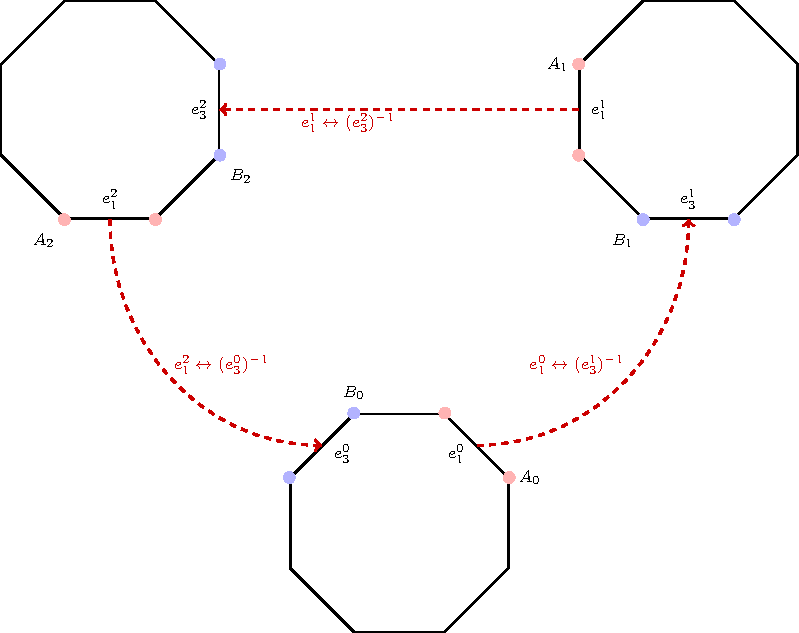
\includegraphics[width=0.8\textwidth]{images/group-symmetry}
    \caption{The octagons $P_2^0$, $P_2^1$, and $P_2^2$ with their edges and vertices labeled according to the gluing rules.}
    \label{fig:octagons}
\end{figure}

Let $g=4$, so $N=g-1=3$. We use three octagons, $P_2^0$ (octagon 0), $P_2^1$ (octagon 1), and $P_2^2$ (octagon 2). The gluing rules derived from the general formula are:
For $j=0$:
\begin{itemize}
    \item $e_1^0 \leftrightarrow (e_3^{(0+1)\pmod 3})^{-1} \Rightarrow e_1^0 \leftrightarrow (e_3^1)^{-1}$
    \item $e_2^0 \leftrightarrow (e_4^0)^{-1}$
    \item $e_5^0 \leftrightarrow (e_7^0)^{-1}$
    \item $e_6^0 \leftrightarrow (e_8^0)^{-1}$
\end{itemize}
For $j=1$:
\begin{itemize}
    \item $e_1^1 \leftrightarrow (e_3^{(1+1)\pmod 3})^{-1} \Rightarrow e_1^1 \leftrightarrow (e_3^2)^{-1}$
    \item $e_2^1 \leftrightarrow (e_4^1)^{-1}$
    \item $e_5^1 \leftrightarrow (e_7^1)^{-1}$
    \item $e_6^1 \leftrightarrow (e_8^1)^{-1}$
\end{itemize}
For $j=2$:
\begin{itemize}
    \item $e_1^2 \leftrightarrow (e_3^{(2+1)\pmod 3})^{-1} \Rightarrow e_1^2 \leftrightarrow (e_3^0)^{-1}$
    \item $e_2^2 \leftrightarrow (e_4^2)^{-1}$
    \item $e_5^2 \leftrightarrow (e_7^2)^{-1}$
    \item $e_6^2 \leftrightarrow (e_8^2)^{-1}$
\end{itemize}

The calculation of the genus proceeds as follows:
\begin{enumerate}
    \item \textbf{Faces (F)}: We start with $N=3$ octagons, so $F=3$.
    \item \textbf{Edges (E)}: There are $8N = 8 \times 3 = 24$ edges in total before gluing. There are $4N = 4 \times 3 = 12$ gluing relations. Thus, the number of distinct edges after gluing is $E = \frac{24}{2} = 12$.
    \item \textbf{Vertices (V)}:
        For each octagon $P_2^j$ ($j=0,1,2$), the internal gluings (type 2, 3, 4, involving $B_1, A_2, B_2$ where $\phi(X)=\bar{0}$) result in two local vertex classes:
        \begin{itemize}
            \item $G_{jA} = \{v_1^j, v_2^j, v_5^j, v_6^j, v_7^j, v_8^j\}$
            \item $G_{jB} = \{v_3^j, v_4^j\}$
        \end{itemize}
        This gives $2N = 2 \times 3 = 6$ local vertex classes: $G_{0A}, G_{0B}, G_{1A}, G_{1B}, G_{2A}, G_{2B}$.
        The type 1 gluing rules (involving $A_1$ where $\phi(A_1)=\bar{1}$) connect vertices across different octagons:
        \begin{itemize}
            \item $e_1^0 \leftrightarrow (e_3^1)^{-1}$ implies $G_{0A} \sim G_{1B}$.
            \item $e_1^1 \leftrightarrow (e_3^2)^{-1}$ implies $G_{1A} \sim G_{2B}$.
            \item $e_1^2 \leftrightarrow (e_3^0)^{-1}$ implies $G_{2A} \sim G_{0B}$.
        \end{itemize}
        These $N=3$ relations link the $2N=6$ local classes into $N=3$ distinct global vertex classes:
        \begin{itemize}
            \item $VC_0 = G_{0A} \cup G_{1B}$
            \item $VC_1 = G_{1A} \cup G_{2B}$
            \item $VC_2 = G_{2A} \cup G_{0B}$
        \end{itemize}
        Thus, $V=N=3$.
    \item \textbf{Euler Characteristic ($\chi$)}:
    $$ \chi = V - E + F = 3 - 12 + 3 = -6 $$
    \item \textbf{Calculated Genus ($g_{calc}$)}:
    Since the surface is orientable, $\chi = 2 - 2g_{calc}$.
    $$ -6 = 2 - 2g_{calc} \implies 2g_{calc} = 8 \implies g_{calc} = 4 $$
\end{enumerate}
This matches the intended genus $g=4$.

\section{Geometric Realization, Covering Structure, and Fundamental Group Hierarchy}
\label{sec:integrated_discussion}

This section aims to provide a deeper understanding of the key features of the proposed rotational construction for genus $g$ surfaces. We will elaborate on how this construction naturally gives rise to a covering map, its geometric realizability in hyperbolic space, and the profound algebraic relationships it reveals among fundamental groups. The method detailed offers an alternative to the standard procedure of building a genus $g$ surface from a single $4g$-sided polygon, particularly emphasizing a hierarchical relationship and inherent symmetries.

\subsection{The Covering Map $p: S_g \to S_2$ and its Properties}

The core of our construction lies in viewing the genus $g$ surface $S_g$ as an $N=(g-1)$-sheeted regular covering of a genus 2 surface $S_2$, with the cyclic group $Z_N$ acting as the group of deck transformations.

\paragraph{Definition and Deck Transformations.}
The construction inherently defines an $N=(g-1)$-sheeted regular covering map $p: S_g \to S_2$. The deck transformation group is isomorphic to $Z_N = \{\bar{0}, \bar{1}, \ldots, \overline{N-1}\}$. An element $\bar{k} \in Z_N$ acts by mapping the $j$-th octagonal sheet $P_2^j$ to $P_2^{(j+k) \pmod N}$, while preserving the gluing rules. For any point $x \in S_2$, its preimage $p^{-1}(x)$ in $S_g$ consists of $N$ distinct points, one in each octagonal sheet $P_2^j$. These $N$ octagons, when assembled according to the gluing rules, form a fundamental domain for $S_g$, and each sheet $P_2^j$ projects down to $S_2$ via $p$, effectively "covering" the base surface $S_2$.

\paragraph{Monodromy.}
The monodromy action of $\Gamma_2 = \pi_1(S_2)$ on a fiber $p^{-1}(x)$ is determined by the homomorphism $\phi: \Gamma_2 \to Z_N$. For a loop $\gamma \in \Gamma_2$ based at $x_0 \in S_2$, lifting $\gamma$ to a path in $S_g$ starting at a point $y_j \in p^{-1}(x_0)$ (where $y_j$ is in the $j$-th sheet) leads to an endpoint $y_{(j+\phi(\gamma)) \pmod N}$. Thus, a loop $\gamma$ with $\phi(\gamma) = \bar{k}$ induces a cyclic permutation of the sheets by $k$.

\subsection{Fundamental Group Hierarchy and Algebraic Structure}

The covering $p: S_g \to S_2$ establishes a clear hierarchical relationship between the fundamental groups of $S_g$ and $S_2$.

\paragraph{The Exact Sequence.}
The fundamental group of the constructed surface $S_g$, denoted $\Gamma_g = \pi_1(S_g)$, is a normal subgroup of $\Gamma_2 = \pi_1(S_2)$. The quotient group $\Gamma_2/\Gamma_g$ is isomorphic to the deck transformation group $Z_N$. This relationship is captured by the short exact sequence:
\[
1 \to \Gamma_g \to \Gamma_2 \xrightarrow{\phi} Z_N \to 1.
\]
Here, $\Gamma_g = \ker(\phi)$, and its index in $\Gamma_2$ is $N = g-1$.

\paragraph{Generators of $\Gamma_g$.}
The group $\Gamma_g$ is generated by lifts of those loops in $S_2$ whose image under $\phi$ is the identity element $\bar{0} \in Z_N$.
\begin{itemize}
    \item Loops in $S_2$ corresponding to the generators $B_1, A_2, B_2$ (for which $\phi(B_1) = \phi(A_2) = \phi(B_2) = \bar{0}$) lift to closed loops within each sheet of $S_g$. These lifts are elements of $\Gamma_g$.
    \item A loop in $S_2$ corresponding to the generator $A_1$ (for which $\phi(A_1) = \bar{1}$) lifts to a path in $S_g$ connecting a point in sheet $P_2^j$ to a corresponding point in sheet $P_2^{(j+1) \pmod N}$. Iterating such a loop $N$ times (i.e., $A_1^N$) results in a loop in $S_2$ whose image $\phi(A_1^N) = N \cdot \bar{1} = \bar{0}$ in $Z_N$. Thus, $A_1^N$ lifts to a closed loop in $S_g$ and is an element of $\Gamma_g$. Similarly, elements like $A_1 B_1 A_1^{-1}$ (if $\phi(B_1) \neq \bar{0}$ in a different homomorphism choice) would need to be considered based on their image under $\phi$.
\end{itemize}

\paragraph{The Special Role of $\Gamma_2$.}
In the context of this construction, where $S_g$ is built as a specific $Z_{g-1}$-symmetric cover of a fixed $S_2$, the group $\Gamma_2$ acts as a parent group from which a family of groups $\{\Gamma_g\}_{g \ge 2}$ is derived. More broadly, in the lattice of fundamental groups of closed orientable hyperbolic surfaces ordered by subgroup inclusion, $\Gamma_k$ (for genus $k \ge 2$), groups $\Gamma_2$ are maximal elements, as they cannot be proper finite-index subgroups of another $\Gamma_h$ (where $h \ge 2$).

\subsection{The Fundamental Domain $P_g^*$ and Hyperbolic Geometric Realization}

The union of the $N=(g-1)$ octagons in the hyperbolic plane, $P_g^* = \bigcup_{j=0}^{N-1} \alpha_j(P_2)$ (where $P_2$ is a fundamental octagon for $\Gamma_2 = \pi_1(S_2)$, and $\alpha_j$ are appropriately chosen isometries corresponding to the sheets), forms a legitimate fundamental domain for the resulting genus $g$ surface $S_g = \mathbb{H}^2/\Gamma_g$. The gluing rules defined are precisely the side-pairings of this larger domain $P_g^*$ by elements of $\Gamma_g = \ker(\phi)$.

\paragraph{Hyperbolic Realizability.}
The geometric realization of this construction can be grounded in hyperbolic geometry.
We can choose $P_2$ to be a regular octagon in the hyperbolic plane $\mathbb{H}^2$ with each internal angle being $\pi/4$. Such an octagon exists (as $8 \times \pi/4 = 2\pi < (8-2)\pi = 6\pi$). When its 8 sides are paired according to the standard gluing for a genus 2 surface (e.g., $e_1 \leftrightarrow e_3^{-1}, e_2 \leftrightarrow e_4^{-1}, e_5 \leftrightarrow e_7^{-1}, e_6 \leftrightarrow e_8^{-1}$), all 8 vertices of $P_2$ are identified to a single point in $S_2$. The sum of the angles around this point is $8 \times (\pi/4) = 2\pi$, satisfying the angle condition of Poincaré's polygon theorem for $P_2$ to be a fundamental domain for $S_2$. The Bolza surface is a prime example of a genus 2 surface admitting such a regular octagonal fundamental domain.

Now, consider the fundamental domain $P_g^* = \bigcup_{j=0}^{N-1} P_2^j$ formed by $N$ such identical regular octagons $P_2^j$, arranged and glued according to our $Z_N$-symmetric rules. As established in our vertex analysis (Section 3, item 3), the $8N$ initial vertices are grouped into $N$ distinct equivalence classes in $S_g$. Each such vertex class in $S_g$ is formed by exactly 8 original "corners" from the constituent octagons. If each of these 8 corners contributes an angle of $\pi/4$, the total angle sum around each of the $N$ distinct vertices in $S_g$ is $8 \times (\pi/4) = 2\pi$. This satisfies the angle condition of Poincaré's polygon theorem for $P_g^*$ to be a fundamental domain for $S_g = \mathbb{H}^2/\Gamma_g$. Thus, the constructed surface $S_g$ can be realized as a hyperbolic surface with a metric derived from this tessellation.

\paragraph{Relation to the $4g$-gon.}
While the canonical fundamental domain is often presented as a $4g$-gon, $P_g^*$ is a polygon (formed by $N$ adjoined octagons) whose boundary edges are identified by $\Gamma_g$ to yield $S_g$. $P_g^*$ can be transformed into a standard $4g$-gon via topological cutting and pasting operations.

\paragraph{Holonomy Representation.}
When $P_2$ is chosen as a regular hyperbolic octagon (like that for the Bolza surface), the monodromy action described earlier directly corresponds to the holonomy representation of the resulting hyperbolic structure on $S_g$. The deck transformations $Z_N$ manifest as isometries of $S_g$.

\subsection{Flexibility and Generalizations of the Construction}

The specific choice of homomorphism $\phi$ and the nature of the quotient group $Z_N$ offer avenues for variations and generalizations.

\paragraph{Dependence on the Homomorphism $\phi$.}
Our chosen homomorphism $\phi(A_1) = \bar{1}, \phi(B_1) = \phi(A_2) = \phi(B_2) = \bar{0}$ is not unique. Different surjective homomorphisms $\phi': \Gamma_2 \to Z_N$ will generally lead to different covering spaces $S_g'$.
\begin{itemize}
    \item For instance, if one chose $\phi'(B_1) = \bar{1}$ and $\phi'(A_1) = \phi'(A_2) = \phi'(B_2) = \bar{0}$, the gluing rule for edge $e_2^j$ would become $e_2^j \leftrightarrow (e_4^{(j+1) \pmod N})^{-1}$. This would alter the vertex identification cycles and potentially the geometric properties of the resulting surface $S_g'$ (e.g., its full isometry group), even though its genus, as determined by the Euler characteristic calculation based on $N$ octagons, would remain $g = N+1$.
    \item The genus of the resulting surface is invariant under such choices (as long as $\phi$ is surjective and $N=g-1$), but geometric features, such as the lengths of shortest geodesics or the full automorphism group of $S_g$, may differ.
\end{itemize}

\paragraph{Generalizations to Non-Cyclic Covers.}
While this note has focused on cyclic covers ($Z_N$), the general principle of constructing $S_g$ from $N$ copies of $P_2$ can be extended to situations where $\Gamma_g$ is a normal subgroup of $\Gamma_2$ such that $\Gamma_2/\Gamma_g \cong G$, where $G$ is any finite group of order $N$.
\begin{itemize}
    \item If $G$ is a non-abelian group, the covering $S_g \to S_2$ would be regular but not necessarily cyclic. The $N$ sheets would correspond to the elements of $G$, and the gluing rule for an edge $e_i^x$ (in sheet $x \in G$) paired by $X \in \Gamma_2$ would be $e_i^x \leftrightarrow (e_k^{x \cdot \phi(X)})^{-1}$ (or $e_k^{\phi(X) \cdot x}$ depending on convention).
    \item The genus calculation via Euler characteristic remains valid ($F=N$, $E=4N$, leading to $V=N$ for $\chi = 2-2N = 2-2g$), but the specific vertex and edge identification patterns would be more complex, reflecting the structure of $G$.
\end{itemize}
This highlights that $S_2$ can serve as a base for constructing a rich variety of higher genus surfaces with diverse symmetry groups.

\section{Conclusion}
This note presents a novel rotational construction of genus \(g\) surfaces from \((g-1)\) octagons, leveraging the hierarchical relationship between surfaces of different genera. By interpreting \(S_g\) as a \(Z_N\)-symmetric covering of a genus 2 surface \(S_2\), we derive explicit gluing rules for assembling \(S_g\) from \(N\) octagonal fundamental domains. Key contributions include:
\begin{enumerate}
    \item \textbf{Constructive Framework}: A systematic method to build \(S_g\) via cyclic covers, validated by Euler characteristic calculations.
    \item \textbf{Geometric Realization}: Demonstration that \(S_g\) admits a hyperbolic metric when the base octagon \(P_2\) is regular (e.g., Bolza surface), satisfying Poincaré's polygon theorem.
    \item \textbf{Fundamental Group Insights}: Clarification of the subgroup hierarchy \(\Gamma_g \triangleleft \Gamma_2\) and the role of homomorphisms \(\phi: \Gamma_2 \to Z_N\) in defining covers.
\end{enumerate}

This approach offers pedagogical and practical advantages:
\begin{itemize}
    \item \textbf{Visualization}: The cyclic gluing of octagons provides an intuitive model for higher-genus surfaces.
    \item \textbf{Hierarchy Emphasis}: \(S_2\) serves as a "building block" for symmetric \(S_g\), contrasting with the standard \(4g\)-gon construction.
    \item \textbf{Computational Utility}: The method simplifies genus calculations and generalizes to irregular covers.
\end{itemize}

Future work could explore:
\begin{itemize}
    \item \textbf{Alternative Homomorphisms}: Classifying covers arising from different \(\phi\) and their geometric properties.
    \item \textbf{Higher Symmetries}: Extending the construction to surfaces with larger automorphism groups (e.g., Hurwitz surfaces).
    \item \textbf{Applications}: Using this framework to study spectral theory or heat kernels on symmetric hyperbolic surfaces.
\end{itemize}

In summary, this rotational construction enriches the tapestry of surface topology, highlighting the genus 2 surface as a foundational element in the architecture of higher-genus spaces.

\end{document}